\chapter{مفاهیم پایه}
در این فصل به توضیح و مرور مفاهیم مقدماتی و پایه‌ای مرتبط با این پروژه می‌پردازیم. با توجه به اینکه بخشی از روش مورد استفاده برمبنای شبکه عصبی پیچشی بوده و همچنین در قسمت ارزیابی از یک مدل دنباله به دنباله استفاده می‌شود، توضیحاتی در مورد شبکه‌های عصبی در انتهای این بخش ارائه خواهد شد.
\section{پردازش زبان طبیعی}
پردازش زبان طبيعی\footnote{\lr{Natural Language Processing}} يکی از زيرشاخه‌های مهم حوزه‌ی هوش مصنوعی و دانش زبان‌شناسی‌ است. تلاش عمده در اين زمينه، ایجاد توانایی درک مفاهیم بیان شده در یک زبان طبیعی برای یک ماشین می‌باشد که می‌توان آنرا به دو قسمت پردازش زبان گفتار و نوشتار تقسیم نمود. با ورود فناوری رایانه‌ای به زندگی بشر، پردازش زبان طبیعی از مهمترین امور مورد توجه بوده است.
برای ایجاد توانایی فهم زبان طبیعی توسط ماشین نیاز به دانش وسیعی از زبان می‌باشد که موجب نیاز به دانش زبان‌شناسان علاوه بر محققان علوم رایانه می‌گردد.
کاربردهای پردازش زبان طبیعی به دو دسته‌ی کاربردهای نوشتاری و کاربردهای گفتاری قابل تقسیم است. از کاربردهای نوشتاری آن می‌توان به استخراج اطلاعاتی خاص از یک متن، ترجمه یک متن به زبانی دیگر یا یافتن مستنداتی خاص در یک پایگاه داده نوشتاری و از کاربردهای گفتاری آن می‌توان به سرویس‌های خودکار ارتباط با مشتری از طریق تلفن و سیستم‌های کنترلی توسط صدا اشاره کرد. سیستمی که در این پروژه بررسی می‌شود، از دسته‌ی کاربردهای نوشتاری این زمینه می‌باشد.
\section{بازیابی اطلاعات}
به استخراج اطلاعات مورد نیاز از یک منبع اطلاعاتی، بازیابی اطلاعات\footnote{\lr{Information Retrieval}} می‌گویند. این استخراج بر پایه‌ی یک جستجو انجام می‌شود که می‌تواند روی کل داده‌های متنی، فراداده‌ها و یا پایگاه‌های داده انجام گیرد. سیستم مورد بررسی در این پروژه از یک گراف دانش به عنوان منبع اطلاعات استفاده کرده و بوسیله‌ی کوئری‌های \lr{SPARQL} اطلاعات مورد نیازش را از آن استخراج می‌کند.
\section{گراف دانش}
گراف‌های دانش مجموعه‌ی بزرگی از موجودیت‌\footnote{\lr{Entity}}های بهم مرتبط هستند که به وسیله‌ی برچسب‌های معنایی غنی شده‌اند. در واقع گراف دانش، پایگاه دانشی از حقیقت‌ها\footnote{\lr{Facts}} راجع به موجودیت‌هاست که از جمله‌ی آن‌ها می‌توان به ویکی‌دیتا\footnote{\lr{Wikidata}}، فریبیس\footnote{\lr{Freebase}} و یاگو\footnote{\lr{Yago}} اشاره کرد که معمولا از دانشنامه‌هایی مانند ویکی‌پدیا\footnote{\lr{Wikipedia}}، جئونیمز\footnote{\lr{GeoNames}} و وردنت\footnote{\lr{WordNet}} استخراج می‌گردند. از زمینه‌هایی که گراف دانش در آن‌ها کاربرد دارد می‌توان به موتورهای جستجو، پردازش زبان‌های طبیعی، استخراج آزاد اطلاعات و سامانه‌های پرسش و پاسخ اشاره کرد. بسیاری از سیستم‌های اطلاعاتی روی وب که نیازمند دسترسی به دانش ساخت‌یافته می‌باشند، از گراف دانش استفاده می‌کنند. وب معنایی\footnote{\lr{Semantic Web}} در ابتدا دانش را بر مبنای گراف ارائه نمود که گره‌های آن، موجودیت‌ها و یال‌های آن رابطه‌ی میان موجودیت‌ها می‌باشند. با مطرح شدن داده‌های پیوندی\footnote{\lr{Linked Data}}، اتصال مجموعه داده‌های مختلف به یکدیگر در وب معنایی عنوان شد. بنابراین آینده‌ی وب معنایی، یک پایگاه دانش جهانی بسیار بزرگ و مستقل از زبان شامل موجودیت‌هایی است که به‌طور معنایی به‌هم مرتبط شدند.\\
اساس وب معنایی، مدل داده‌ای چارچوب توصیف منابع\footnote{\lr{Resource Description Framework}} یا به اختصار \lr{RDF} است. در فناوری وب معنایی، بیشتر داده‌ها از قبیل داده‌های پیوندی، به‌صورت \lr{RDF} ذخیره و نمایش داده می‌شوند. از این جهت شاید بتوان گفت که مدل داده‌ای وب معنایی، \lr{RDF} هست. در \lr{RDF} هر منبع یا موجودیت دارای یک شناسه به‌ عنوان نام یا آدرس یکتا است. این آدرس یکتا باید از طریق پروتکل \lr{HTTP} قابل جستجو بوده و اطلاعات مفیدی را به شکل استاندارد فراهم نماید. این مدل، همانند مدل داده‌ای جدولی در پایگاه‌های داده‌ای رابطه‌ای نیست، همچنین مانند ساختار درختی \lr{XML} نیز نیست بلکه \lr{RDF} یک گراف است. داده‌های وب معنایی معمولا به صورت سه‌تایی\footnote{\lr{Triple}} توصیف می‌شوند که شامل سه جزء فاعل\footnote{\lr{Subject}}، گزاره\footnote{\lr{Predicate}} و مفعول\footnote{\lr{Object}} است \cite{persian_graph}.\\
هر سه‌تایی را می‌توان به ‌صورت یک زنجیر گره-یال-گره مانند شکل \ref{fig:rdf-strcutre} نمایش داد. به‌عنوان مثال حقیقتی مانند «پایتخت ایران شهر تهران است» را می‌توان به ‌صورت یک سه‌‌تایی توصیف نمود. این توصیف براساس ساختار انتزاعی مذکور، در شکل ‌\ref{fig:rdf-sample} نمایش داده شده‌ است.

\begin{multicols}{2}
\begin{figure}[H]
	\centering
	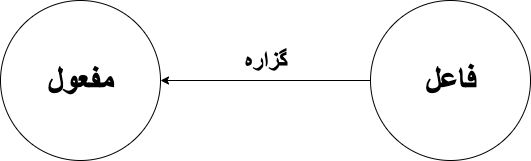
\includegraphics[scale=0.375]{figures/rdf/structure.png}
	\caption[ساختار انتزاعی گراف \lr{RDF}]{ساختار انتزاعی گراف \lr{RDF}}
	\label{fig:rdf-strcutre}
\end{figure}
	\columnbreak
\begin{figure}[H]
	\centering
	
\includegraphics[scale=0.375]{figures/rdf/sample.png}
	\caption[نمونه‌ای از یک سه‌تایی \lr{RDF}]{نمونه‌ای از یک سه‌تایی \lr{RDF}}
	\label{fig:rdf-sample}
\end{figure}
\end{multicols}

\section{سیستم پرسش و پاسخ}
سیستم‌ پرسش و پاسخ\footnote{\lr{Question Answering System}} به سیستمی گفته می‌شود که بتواند سوالات مطرح شده توسط یک انسان در زبان طبیعی را بررسی کرده و به آن به صورت خودکار پاسخ دهد. اینگونه سیستم‌ها در زمینه‌ی پردازش زبان طبیعی و بازیابی اطلاعات بررسی می‌شوند.\\
یک روش دسته‌بندی سیستم‌های پرسش و پاسخ مبتنی بر گراف دانش، بر اساس تعداد روابطی از گراف است که برای پاسخ‌دهی به سوال استفاده می‌شود. \\
دسته اول سوالات ساده هستند که برای پاسخ‌دهی به این سوالات فقط نیاز به یک رابطه از گراف دانش می‌باشد. به عنوان مثال در سوال "نام آثار سعدی چه هستند؟" با بررسی رابطه‌ی "آثار" از موجودیت "سعدی" در گراف دانش می‌توان پاسخ‌های این سوال را استخراج نمود. سیستمی که در این پروژه بررسی می‌شود از این دسته می‌باشد.\\دسته دوم سوالات پیچیده هستند که برای پاسخ دادن به آنها به بیش از یک رابطه از گراف دانش نیاز است. به عنوان مثال برای پاسخ دادن به سوال "علی دایی در کدام تیم‌های لیگ آلمان بازی کرده است؟" ابتدا باید رابطه‌ی "باشگاه" از موجودیت "علی دایی" بررسی شده و سپس رابطه‌ی "لیگ" روی هر کدام از نتایج رابطه‌ی اول بررسی شود.

\section{شبکه‌‌های عصبی}
در این قسمت به توضیح شبکه‌های عصبی و پایه‌ی ریاضی آنها و همچنین تشابه آنها با ریشه‌ی زیستی و طبیعی این شبکه‌ها پرداخته می‌شود. در ادامه نیز با انواعی از اینگونه شبکه‌ها آشنا خواهیم شد.
یکی از روش‌های نوین در یادگیری‌ ماشینی\footnote{\lr{Machine Learning}}، شبکه‌های عصبی یا به عبارتی شبکه‌های عصبی مصنوعی\footnote{\lr{Artificial Neural Networks}} بوده که می‌توان از آنها برای برای اعمال دانش بدست آمده از سامانه‌های پیچیده استفاده نمود. ساختار این شبکه‌ها مشابه ساختار زیستی مغز طبیعی بوده و از آن الهام گرفته است.
هسته‌ی اصلی پردازشی این شبکه‌ها نرون‌های مصنوعی‌‌\footnote{\lr{Artificial Neurons}} هستند که در شمار فراوان در این شبکه‌ها ظاهر شده و می‌توانند‌ به صورت کاملا به‌هم‌پیوسته\footnote{\lr{Fully Connected}} یا غیرکاملا به‌هم‌پیوسته\footnote{\lr{Not Fully Connected}} کنار هم قرار گیرند. در شبکه‌های طبیعی، ارتباطات کاملا به‌هم‌پیوسته بوده و در صورت آسیب دیدن یک نرون، نرون دیگری می‌تواند کار آن‌را به ‌عهده بگیرد. 
نرون‌های مصنوعی همانند گونه‌ی طبیعی خود قابلیت یادگیری دارند. یادگیری یک شبکه عصبی مصنوعی میتواند به صورت با نظارت\footnote{\lr{Supervised Learning}} و یا بدون نظارت\footnote{\lr{Unsupervised Learning}} انجام گیرد. شبکه‌هایی که در ادامه بررسی می‌شوند تحت روش یادگیری با نظارت آموزش می‌بینند.
\subsection{تعریف پایه}
یک شبکه‌ی عصبی دارای چندین لایه از نرون‌ها می‌باشد. عموما هر شبکه دارای سه لایه‌ی اصلی ورودی، پردازش و خروجی است. به طور معمول نرون‌های هر لایه به تمامی نرون‌های لایه‌های قبل و بعد خود متصل می‌شود مگر آنکه به طور مخصوص این ارتباط محدود گردد. در عین حال هیچ نرونی با نرون‌های هم‌لایه‌ی خود اتصالی برقرار نمی‌کند. نرون کوچکترین واحد پردازشگر در شبکه است و یک شبکه مجموعه‌ای از نرون‌ها می‌باشد که با معماری خاصی کنار هم قرار گرفته و متصل شده‌اند. رفتار یک شبکه حاصل از مجموع رفتار همگی نرون‌های آن شبکه است که به طور مستقل در حال پردازش می‌باشند. هر نرون می‌تواند یک تابع ریاضی خطی یا غیرخطی باشد. در نتیجه یک شبکه‌ی عصبی می‌تواند روابط ریاضی بسیار پیچیده‌ای را برای استفاده فراهم نماید.
\subsection{شبکه‌های عصبی پرسپترون و پرسپترون چندلایه}
پرسپترون ساده‌ترین نوع شبکه‌های عصبی است که یک دسته‌بند دو‌دویی\footnote{\lr{Binary Classifier}} به‌شمار می‌آید. فرض کنید که ورودی‌های شبکه‌ی عصبی $d$ بعدی بوده و به‌تعداد $n$ داده در اختیار داشته باشیم. در این صورت یک پرسپترون ورودی‌ خود $x \in R^{d}$ را به مقدار خروجی $f(x) \in R$ با رابطه‌ی زیر تبدیل می‌کند: 

\begin{equation}
\label{eqn:perceptron}
	f(x) = \begin{cases}
	1 & \ \ if \ <w, x> +\ b > 0 \\
	0 & \ \ otherwise
	\end{cases}
\end{equation}

که مقدار $w \in R^d$ بردار وزن  شبکه و $b$ نشان‌دهنده‌ی بایاس آن است که وظیفه‌ی آن جابجایی مرز تصمیم‌گیری از مبدا است. نماد $<w,x>$ نشان‌دهنده‌ی ضرب داخلی دو بردار است که مقدار آن برابر با $\sum_{i=1}^{m}w_i x_i$ می‌باشد.
طی مرحله‌ی یادگیری، شبکه‌ی پرسپترون تلاش می‌کند تا با توجه به داده‌هایی که در اختیار میگیرد، مقدار بهینه برای بردار وزنش یا همان $w$ و مقدار بایاسش یا همان $b$ را پیدا کند.
\subsubsection{پرسپترون‌ چند‌لایه}
یک پرسپترون چند‌لایه\footnote{\lr{Multi-Layer Perceptron}} شامل حداقل سه‌لایه ورودی، پردازش(پنهان) و خروجی می‌باشد. در واقع هر‌ شبکه‌ی عصبی با سه‌لایه یا بیشتر به یک پرسپترون چندلایه‌ نام‌گذاری می‌شود. برای مثال در شکل \ref{fig:perceptron} نمایشی از یک‌ شبکه‌ی پرسپترون با دو‌لایه‌ی پنهان آمده است. 
\begin{figure}[h]
	\centering
	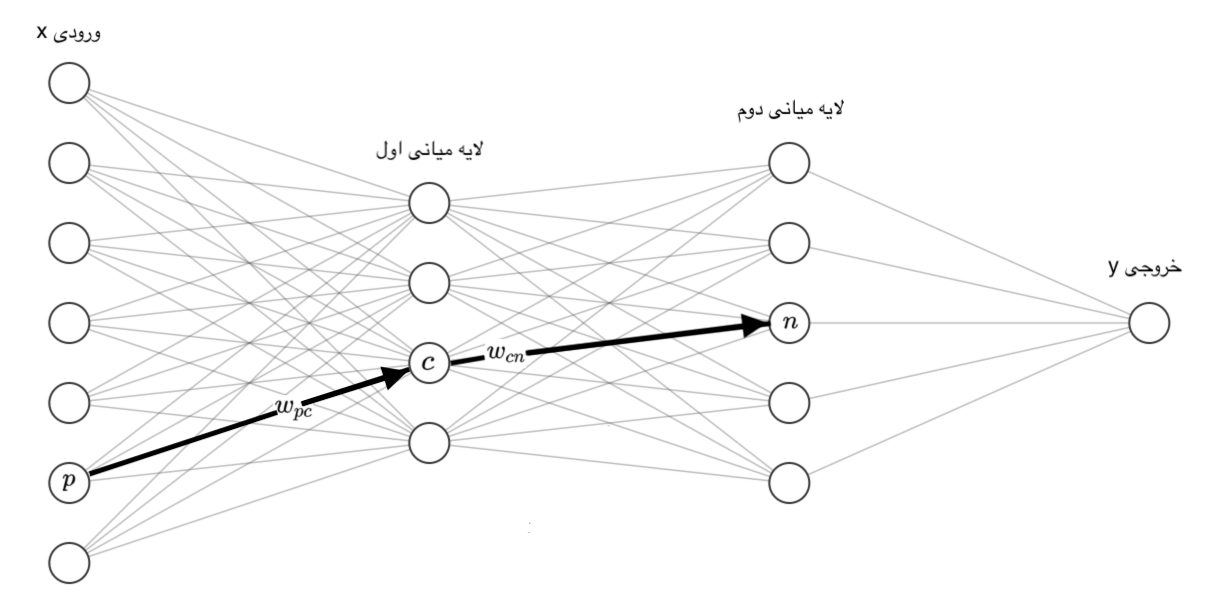
\includegraphics[scale=0.7]{figures/ml-perceptron.png}
	\caption[اتصالات یک شبکه‌ی عصبی پرسپترون با دو لایه‌ی پنهان]{اتصالات یک شبکه‌ی عصبی پرسپترون با دو لایه‌ی پنهان. گرادیان وزن‌های هر لایه وابسته به گرادیان وزن‌های لایه‌ی بالاتر می‌باشد.}
	\label{fig:perceptron}
\end{figure}
مقدار خروجی از نرون $p$ را با $b_p$ و وزن شبکه از نرون $p$ به $c$ را با $w_{pc}$ نمایش می‌دهیم. همانطور که در شکل \ref{fig:perceptron} مشخص است، نرون $c$ مقادیر تمامی نرون‌های لایه‌ی ورودی را دریافت کرده و روی آنها پردازش انجام می‌دهد. مجموع ضرب ورودی‌های نرون‌ $c$ با وزن‌هایشان را با $a_c$ نمایش می‌دهیم:
\begin{equation}
	a_c = \sum_{p}^{} w_{pc} b_{p}
\end{equation}
حال جهت ایجاد امکان مدل‌کردن روابط غیر‌خطی در ورودی‌ها، باید روی $a_c$ تابعی غیرخطی اعمال شود. در این صورت خواهیم داشت:
\begin{equation}
	b_c = \theta_c (a_c)
\end{equation}
که در آن $\theta_c$ تابع غیر‌خطی اعمال شده و $b_c$ خروجی جدید بدست‌آمده است. حال اگر تمامی‌ وزن‌های شبکه‌ی پرسپترون‌ را با $W$ نمایش دهیم و خروجی شبکه پرسپترون به ازای داده‌ی $x_i$ را $h_W(x_i)$ فرض کنیم، تابع هدف به‌صورت:
\begin{equation}
	Q(W) = \sum_{i = 1}^{n} l(h_W(x_i), y_i)
\end{equation}
خواهد بود که برای $l$ می‌توان از خطای‌ مربعات\footnote{\lr{Least Squared Error}} و یا منفی لگاریتم درست‌نمایی\footnote{\lr{Negative Log Likelihood}} استفاده کرد. 

برای بدست آوردن کمینه‌ی $Q(W)$ باید از روش گرادیان کاهشی\footnote{\lr{Gradient Descent}} استفاده کرد.  به این معنی که گرادیان تابع را حساب کرده، کمی در خلاف جهت آن حرکت کرده و این کار را آنقدر ادامه داد تا تابع هزینه خیلی کوچک شود. روش انتشار معکوس\footnote{\lr{Backpropagation}} در واقع روشی برای پیدا کردن گرادیان تابع $Q(W)$ نسبت به تمامی وزن‌های شبکه می‌باشد.

\subsection{شبکه‌ی عصبی پیچشی}
شبکه‌های پرسپترون چندلایه که در بخش قبل معرفی شدند با آنکه قابلیت یادگیری روی داده‌های غیرخطی را دارند اما در مسائلی با داده‌های حجیم مانند تصاویر دچار مشکل شده و با چنین ساختاری نیاز به تعداد پارامترهای زیادی دارند که موجب مشکل شدن فرایند یادگیری در اینگونه مسائل خواهد شد. برای رفع این مشکل از مفهوم و عملیات کانولوشن\footnote{\lr{Convolution}} استفاده شده و شبکه‌هایی با نام شبکه‌ی عصبی پیچشی\footnote{\lr{Convolutional Neural Network}} معرفی می‌شوند. عملیات پایه‌ای اینگونه شبکه‌ها عملیات کانولوشن می‌باشد. در این ساختار تعدادی هسته یا فیلتر وجود دارد که به آنها هسته‌ی لغزشی گفته می‌شود. این هسته‌ها همانند عملیات کانولوشن بر روی هر قسمت از داده‌ها قرار گرفته و پردازش انجام می‌دهند و این کار را روی همه‌ی قسمت‌های تصویر تکرار می‌کنند. هرکدام از این هسته‌ها دارای وزن‌هایی هستند که در مرحله‌ی یادگیری مورد آموزش قرار می‌گیرند. رابطه‌ی \ref{eqn:conv_rel} نشان دهنده‌ی این عملیات است. در این رابطه $x$ تصویر ورودی، $y$ ترم بایاس، $K$ اندازه‌ی هسته لغزشی،  $w$ وزن‌های آموزش (هسته‌ی لغزشی) و $z_{i, j}$ خروجی عملیات کانولوشن است. 
\begin{equation}
\label{eqn:conv_rel}
	Z_{i,j} = y_{i, j} + \sum_{m=0}^{K-1}\sum_{n=0}^{K-1}x_{i+m, j+n}w_{m,n}
\end{equation}

ترکیب این عملیات با اعمالی که در ادامه به آنها اشاره می‌کنیم،  شبکه‌ی عصبی با قابلیت بالا در پردازش تصاویر را نتیجه خواهد داد. این اعمال عبارتند از:
\begin{itemize}
	\item پولینگ\footnote{\lr{Pooling}}:
	عمل پولینگ یکی از اعمال اصلی شبکه‌های عصبی پیچشی بوده و به طور معمول  از آن استفاده می‌شود. از این عملیات برای کاهش بعد داده هنگام پردازش استفاده می‌شود. این عمل روی قسمت‌های مختلف داده قرار گرفته و داده‌های آن قسمت را یکی می‌کند. برای انجام آن روش‌های مختلفی وجود دارد که از انواع آن می‌توان به پولینگ بیشینه\footnote{\lr{Max Pooling}} و پولینگ میانگین\footnote{\lr{Average Pooling}} اشاره نمود. از مزیت‌های این عملیات بی‌اثر کردن شبکه عصبی پیچشی نسبت به تغییرات تصاویر نظیر حرکات انتقالی \footnote{\lr{Translation}}  می‌باشد.
	
	\item توابع فعال‌ساز غیر‌خطی\footnote{\lr{Non-Linear Activation Functions}}:
	 این توابع مختص شبکه‌های پیچشی نیستند و در شبکه‌های پرسپترون نیز از قابلیت غیر‌خطی‌ای که فراهم ‌می‌کنند استفاده می‌شود، هرچند کاربرد آنها در شبکه‌های عصبی پیچشی اهمیت بسیار بالایی پیدا می‌کند. از جمله مهمترین توابع فعال‌ساز غیر‌خطی مورد استفاده در شبکه‌های عصبی پیچشی می‌توان به تابع خطی رقیق شده\footnote{\lr{Rectified Linear Unit}} یا به‌طور اختصاری \lr{ReLU} اشاره داشت. ویژگی خاص این تابع که نمودار آن در \ref{fig:relu} نشان داده شده است در این است که در عین حال که غیرخطی بوده و می‌تواند یه یادگیری الگوهای پیچیده غیرخطی کمک کند، پردازش آن راحت بوده و مشتق آن بسیار ساده محاسبه می‌شود و استفاده از آن به‌صرفه‌تر از توابع غیرخطی‌ای نظیر تانژانت هایپربولیک\footnote{\lr{Tanh}} می‌باشد.
\end{itemize}

\begin{figure}[t!]
	\centering
	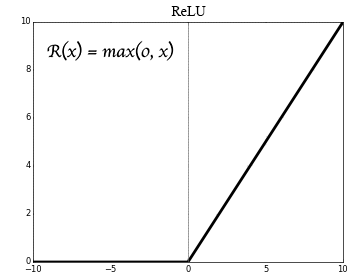
\includegraphics[scale=0.55]{figures/relu.png}
	\caption[نمودار تابع فعال‌ساز غیرخطی \lr{ReLU} مورد استفاده در شبکه‌های پیچشی]{نمودار تابع فعال‌ساز غیر‌خطی \lr{ReLU} مورد استفاده در شبکه‌های پیچشی‌}
	\label{fig:relu}
\end{figure}

\begin{figure}[t!]
	\centering
	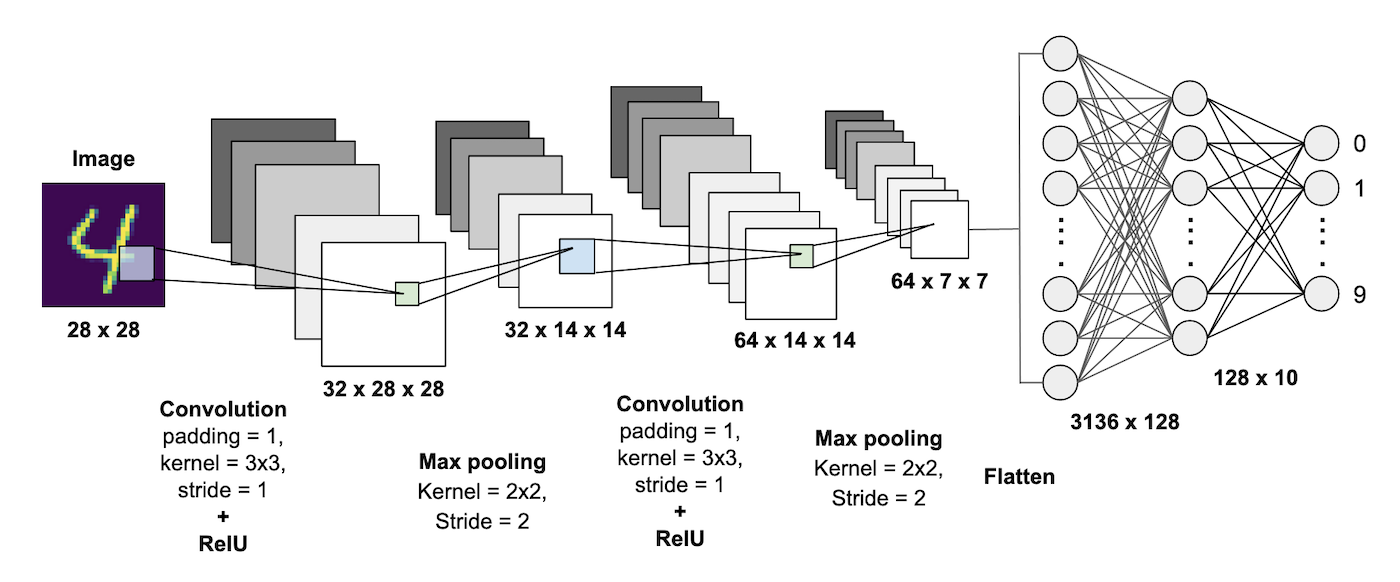
\includegraphics[scale=0.3]{figures/cnn-handwriting.png}
	\caption[معماری کلی یک شبکه‌ی عصبی پیچشی]{معماری کلی یک شبکه‌ی پیچشی در دسته‌بندی اعداد دست‌نوشته}
	\label{fig:cnn}
\end{figure}
نهایتا با ترکیب عملیات کانولوشن و پولینگ، و تکرار این امر در زمان آموزش، هسته‌های شبکه‌ی پیچشی مانند الگوریتم‌های مبتنی بر هسته‌های دست‌ساز در پردازش تصاویر یادگرفته و عمل می‌کنند. به عنوان مثال، در دسته‌بندی تصاویر چهره‌ی انسان، هسته‌هایی برای شناسایی رنگ مو، حالت ابرو و حالت بینی چهره شکل میگیرد. این ویژگی‌ها با اینکه به لطف عملیات پولینگ ابعاد پایینی دارند اما برای تشخیص چهره بسیار کاربردی بوده و استفاده می‌شوند. بنابراین در انتهای شبکه عصبی پیچشی از یک دسته‌بند مبتنی بر شبکه عصبی برای تشخیص خروجی استفاده می‌شود. نمونه‌ی چنین شبکه‌ای را که برای تشخیص اعداد دست‌نوشته استفاده می‌شود، در شکل \ref{fig:cnn} مشاهده می‌کنید. با توجه به وجود ۱۰ کلاس مختلف در مسئله‌ی تشخیص عدد دست‌نوشته، لایه‌ی دسته‌بند این شبکه که در انتهای آن قرار دارد دارای طول ۱۰ می‌باشد \cite{patel2019mnist}.
\subsection{شبکه‌‌ی عصبی بازگشتی}
ضعفی که در شبکه‌های معرفی شده در قسمت‌های قبل وجود دارد، ثابت بودن طول داده‌ی ورودی این شبکه‌ها می‌باشد.
در برخورد با داده‌های زبانی، صوت و یا فیلم، توالی و ترتیب اطلاعات اهمیت بالایی پیدا می‌کند. شبکه‌ی بازگشتی\footnote{\lr{Recurrent Neural Network}} این امکان را به ما می‌دهد تا یک توالی با طول نامشخص را به یک بردار با اندازه ثابت بازنمایی کنیم و در عین حال بسیاری از خواص نحوی و ساختاری توالی ورودی را حفظ کنیم. به طور کلی یک شبکه‌ی بازگشتی تابعی است که یک ورودی با طول غیرثابت (مثلا جمله) را به صورت دنباله‌ای از $n$ بردار با ابعاد $R^{d_{in}}$ دریافت و یک بردار خروجی $y$ با ابعاد $R^{d_{out}}$ باز می‌گرداند. رابطه‌ی زیر این موضوع را به‌خوبی بیان می‌کند:
\begin{equation}
\label{eqn:RNN}
	y_{n} = RNN(x_{1: n})
\end{equation}
که در آن $x_{1:n}$ جمله (دنباله) ورودی و $y_n$ بردار خروجی است. شکل \ref{fig:rnn} نمایشی از یک شبکه‌ی عصبی بازگشتی با سلول‌های حافظه‌ای ساده است. در واقع این شبکه از دو بخش اصلی تشکیل شده است:\\

\begin{enumerate}
	\item \textbf{بخش بازگشتی}:
	 این بخش با رابطه‌ی زیر نشان داده‌ می‌شود و به آن حالت درونی یا پنهان شبکه در زمان $t$ نیز گفته می‌شود:
	\begin{equation}
	\label{recursion}
		s_t = R(x_t, s_{t-1})
	\end{equation}
	\item \textbf{خروجی}:
	 که با اعمال تابع فعال‌ساز بر حالت بخش بازگشتی بدست می‌آید:
	\begin{equation}
	\label{output}
		o_t = O(s_t)
	\end{equation}
\end{enumerate}
به طور خلاصه، شبکه بازگشتی هر کلمه را به یک بردار $y_i$ تبدیل می‌کند ولی چون بردار مرحله آخر برگرفته از تمام اطلاعات قبلی است از آن به عنوان بازنمایی جمله استفاده می‌شود.
\begin{figure}[t!]
	\centering
	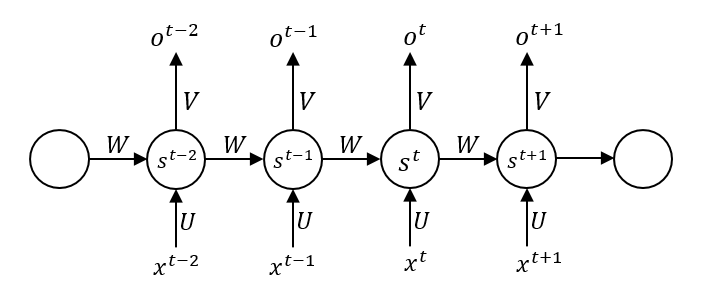
\includegraphics[scale=0.7]{figures/rnn.png}
	\caption[معماری کلی یک شبکه‌ی عصبی بازگشتی]{نمایی از معماری کلی یک شبکه‌ی عصبی بازگشتی متشکل از حالت‌های پنهان و خروجی‌ها}
	\label{fig:rnn}
\end{figure}

روابط \ref{recursion} و \ref{output} را به‌طور دقیق‌تر می‌توان اینگونه‌ بیان کرد:
\begin{equation}
s_t = tanh(Ws_{t-1} + Ux_{t-1})
\end{equation}
\begin{equation}
	o_t = y_t = softmax(Vs_t)
\end{equation}
واضح است که خروجی‌ زمان $t$ در یک شبکه‌ی عصبی بازگشتی به ورودی‌ها و حالت‌های پنهان زمان‌های قبلی وابسته است. به‌همین علت،‌ برای محاسبه‌ی گرادیان‌ها (تغییرات خطا نسبت به تغییر وزن‌ها) از الگوریتم انتشار معکوس در زمان\footnote{\lr{Backpropagation Through Time}} استفاده می‌شود. 

\subsection{شبکه‌ی عصبی دنباله به دنباله}
در شبکه بازگشتی بوسیله‌ی یک حلقه بر روی بردار ورودی جلو می‌رفتیم و هر بار یک خروجی ایجاد می‌کردیم. مشکلی که وجود دارد در مواقعی است که بایستی در سطح کل بردار پیش برویم تا شبکه به درستی آموزش ببیند. به طور مثال وقتی بخواهیم مفهوم یک جمله را برداشت کنیم تا انتهای آن باید پیش برویم، بنابراین تنها خروجی و یا وضعیت آخر برای ما مهم است. موردی که یک شبکه‌ی بازگشتی قادر به انجام آن نیست، تولید یک دنباله‌ از خروجی‌ها با توجه به تمامی اطلاعات ورودی می‌باشد. در چنین وضعیتی از یک شبکه‌ی عصبی دنباله به دنباله\footnote{\lr{Sequence to Sequence Neural Network}} استفاده می‌کنیم \cite{sutskever2014seq2seq}.
\subsubsection{ساختار شبکه}
یک شبکه‌ی دنباله به دنباله از ترکیب دو شبکه‌ی بازگشتی ساخته می‌شود. شبکه اول که کدگذار\footnote{\lr{Encoder}} نام دارد، دنباله‌ی بردار ورودی را به یک بردار وضعیت انتهایی تبدیل می‌کند و سپس آنرا به عنوان وضعیت اولیه برای شبکه بازگشتی دوم که کدگشا\footnote{\lr{Decoder}} نام دارد، در نظر می‌گیرد. شبکه‌ی کدگشا با هر گام که جلو می‌رود یک خروجی تولید می‌کند. بدین صورت دنباله‌ی خروجی مورد نظر ساخته می‌شود.
به عنوان مثال یک سیستم ترجمه‌کننده می‌تواند از این شبکه استفاده کند. به این صورت که ابتدا شبکه بازگشتی اول جمله زبان مبدأ را گرفته و آنرا به یک بردار وضعیت که نشان‌دهنده‌ی مفهوم جمله است، تبدیل می‌کند. سپس شبکه بازگشتی دوم این بردار وضعیت را دریافت کرده و جمله زبان مقصد را تولید می‌کند. در شکل \ref{fig:seq2seq} نمونه‌ای از این ماشین را مشاهده می‌کنید.

\begin{figure}[t!]
	\centering
	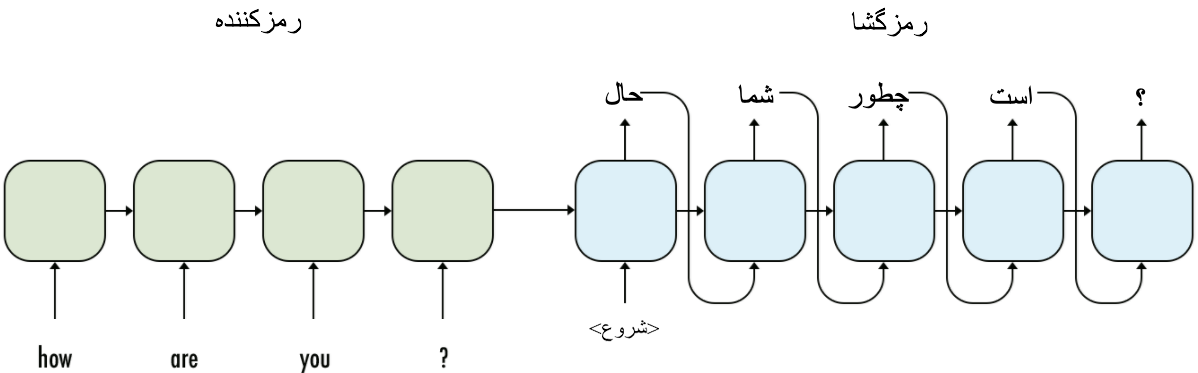
\includegraphics[scale=0.35]{figures/seq2seq.png}
	\caption[نمونه‌ای از شبکه‌ی دنباله به دنباله]{نمونه‌ی یک ماشین ترجمه که از شبکه‌ی دنباله به دنباله تشکیل شده است}
	\label{fig:seq2seq}
\end{figure}

\section{تابع هزینه‌ی \lr{Categorical Cross-Entropy}}
تابع \lr{Categorical Cross-Entropy} یک تابع هزینه\footnote{\lr{Loss Functoin}} مناسب برای دسته‌بندهای تک کلاسه\footnote{\lr{One-Class Classification}} است. دسته‌بندهای تک کلاسه دسته‌بندهایی هستند که هر داده‌ی آنها فقط متعلق به یک کلاس می‌باشد. این تابع هزینه به ازای هر داده بوسیله‌ی رابطه‌ی \ref{eqn:categorical_cross_entropy} بدست می‌آید که در آن $\hat{y}$ نماد بردار احتمالات پیشبینی شده توسط دسته‌بند و $y$ نماد بردار هدف می‌باشد.
\begin{equation}
\label{eqn:categorical_cross_entropy}
L(y, \hat{y}) = - \sum_{i = 0}^{n} (y_i * log(\hat{y}_i))
\end{equation}
